\chapter*{Реферат}                      
\addcontentsline{toc}{chapter}{Реферат} 

\pdfbookmark{Общая характеристика работы}{characteristic}             % Закладка pdf
\section*{Общая характеристика работы}

\newcommand{\actuality}{{\textbf\actualityTXT}}
\newcommand{\progress}{{\textbf\progressTXT}}
\newcommand{\aim}{{\textbf\aimTXT}}
\newcommand{\tasks}{\textbf{\tasksTXT}}
\newcommand{\novelty}{\textbf{\noveltyTXT}}
\newcommand{\influence}{\textbf{\influenceTXT}}
\newcommand{\methods}{\textbf{\methodsTXT}}
\newcommand{\defpositions}{\textbf{\defpositionsTXT}}
\newcommand{\reliability}{\textbf{\reliabilityTXT}}
\newcommand{\probation}{\textbf{\probationTXT}}
\newcommand{\contribution}{\textbf{\contributionTXT}}
\newcommand{\publications}{\textbf{\publicationsTXT}}
\newcommand{\implementation}{\textbf{\implementationTXT}}



{\actuality} Мировые тенденции в области промышленного производства свидетельствуют о том, что современные методы автоматизации и роботизации достигли определенного технологического барьера. Как показала практика, сейчас существенное увеличение производительности, а следовательно, и снижение себестоимости выпускаемой продукции возможно только при постоянном увеличении объемов производства.

Таким образом, в последние десятилетия все средства промышленной автоматизации и роботизации были направлены на массовое производство, способное обеспечить высокое качество выпускаемой продукции при минимальной себестоимости. Однако последние тенденции говорят о том, что массовое производство перестает оправдывать себя. Это связано с тем фактом, что подавляющее большинство современных изделий массового производства включают себя не только физические, но информационные компоненты. Повсеместное развитие средств информатизации и телекоммуникации повлекло за собой появление новых и существенную модернизацию старых изделий. В литературе такие изделия называются <<smart things>> или <<умные вещи>>. 

<<Умные вещи>> являются совокупностью физических и информационных компонентов. Информационные компоненты задают алгоритм работы <<умной вещи>>, позволяют ей осуществлять постоянную самодиагностику и возможность взаимодействия по сети.  Совокупность <<умных вещей>> образует так называемый <<Интернет вещей>>, включающий в себя не только распределенную сеть <<умных вещей>>, но единый облачный сервис для управления ими. Все эти понятия сведенные вместе стали основой новой концепции, именуемой <<кибер-физическая система>>.

Очевидно, что развитие информационных компонентов кибер-физических систем происходит гораздо быстрее, чем физических. Последнее обусловлено более коротким циклом производства программных продуктов в сравнении с физическими объектами, а также более низкой себестоимостью разработки программных продуктов. Вследствие этого возникло определенное технологическое отставание физических компонентов кибер-физических систем по сравнению с информационными.

Как показывает практика, единственным способом избавиться от этого отставания является ускорение темпов промышленного производства за счет более быстрой смены номенклатуры выпускаемых изделий, а также внедрение новых технологических процессов.

Постоянная смена номенклатуры и появление новых видов изделий требуют дополнительных научно-исследовательских и опытно-конструкторских работ, что привело к возникновению нового типа производственных компаний, именуемых малыми инновационными предприятиями (сокр. \textit{МИП}) или стартапами. Цель МИП – непрерывная модернизация существующих, а также проектирование и разработка новых образцов высокотехнологичной продукции в условиях мелкосерийного и единичного производства.

Для достижения поставленной цели МИП должны обладать парком разнообразного оборудования, позволяющего выполнять самые разнообразные технологические операции: от механической обработки изделий и создания электронных компонентов до автоматизированного контроля готовой продукции. Однако большинство МИП не в состоянии обеспечить себя всем необходимым оборудованием и поэтому вынуждены заниматься только разработкой конструкторской документации, передавая производство другим компаниям, обозначаемым термином ОЕМ~(от англ. \textit{Original Equipment Manufacturer}). Принимая во внимание все вышесказанное, необходимо отметить, что такой подход обладает рядом существенных недостатков.

Во-первых, OEM компании в основном заинтересованы в крупных заказах, т.\,к. для них смена номенклатуры связана с необходимостью каждый раз перестраивать производственный процесс. Соответственно, существенная часть времени уходит на технологическую подготовку производства, что значительно повышает себестоимость единицы продукции при работе с малыми партиями. Во-вторых, работа с OEM компаниями увеличивает время вывода на рынок новых видов продукции. Это может быть связано со множеством факторов таких, как необходимость заключения договора на производство и его юридического сопровождения, необходимость согласования конструкторской и технологической документации, передаваемой OEM компании, перегруженность производства OEM компании и т.\,д. В-третьих, риск потери интеллектуальной собственности, связанный с передачей полного комплекта документации на выпускаемые изделия. В-четвертых, OEM компании занимаются только производством по готовой документации, соответственно вопрос создания прототипов изделий, предсерийных образцов и установочных партий изделий для МИП остается нерешенным.

Отдельно стоит отметить, что в рамках Национальной технологической инициативы\footnote{Автономная некоммерческая организация <<Платформа Национальной технологической инициативы>> (сокр. \textit{АНО НТИ}) "--- некоммерческая организация созданная Постановлением председателя Правительства РФ Д.\,А.~Медведева. Разработка НТИ началась в соответствии с поручением Президента России В.\,В.~Путина по реализации послания Федеральному Собранию от 4 декабря 2014 года.} особое внимание уделяется развитию так называемых научно-технологических центров~(сокр. \textit{НТЦ}). Подобные организации реализуют замкнутого цикла исследований и производства. Для подобных организаций также необходимо наличие широкого парка различного технологического оборудования, ведь многие разработки, которые ведутся в НТЦ являются государственной или коммерческой тайной и применение подхода OEM, с передачей конструкторской или технологической документации сторонним фирмам (особенно зарубежным) просто недопустимо.  

Одним из способов решения вышеозначенных проблем является применение модульного технологического оборудования с числовым программным управлением (ЧПУ). Модульное оборудование с ЧПУ представляет собой совокупность независимых модулей, каждый из которых выполняет определенное действие (например, операцию обработки или контроля, перемещение и т.\,д.). На модули накладываются конструктивные параметрические ограничения. Модули объединены единой системой числового программного управления за счет использования стандартизированного и документированного протокола взаимодействия, позволяющего осуществлять децентрализованное взаимодействие как на уровне единицы модульного оборудования, так и на уровне производственной ячейки. 

Модульный принцип построения оборудования с числовым программным управлением освещен в работах таких авторов, как: Аверьянов О.\,И., Светик Дж. (Jozef Svetl\'ik), Йошими И. (Yoshimi Ito) и другие. Также образцы модульного оборудования с ЧПУ выпускаются некоторыми зарубежными и отечественными компаниями. Тем не менее, подавляющее большинство исследований направлены на рассмотрение только конструктивных особенностей и методов проектирования модульного технологического оборудования. Более того, почти все работы связаны исключительно с металлорежущими станками и не рассматривают другие виды обработки.

Также недостаточно проработаны аспекты проектирования и создания гибридного модульного оборудования, включающего в себя несколько видов обработки и/или контроля. Практически не рассматриваются вопросы повышение отказоустойчивости и ремонтопригодности, а также постепенной модернизации технологического оборудования за счёт использования модульного принципа.

Серийно выпускаемые модульные системы являются закрытыми как программно, так и аппаратно, то есть не позволяют в процессе эксплуатации создавать свои модули, равно как и изменять/дополнять программное обеспечение системы числового программного управления. 

Новые подходы к проектированию модульного оборудования требуют совершенствования системы числового программного управления, в частности разработки открытого программного интерфейса и единого протокола взаимодействия модулей, удовлетворяющего требованиям современных телекоммуникационных сетей.

Остается открытым вопрос унификации и стандартизации модульного оборудования. В частности, на сегодняшний день существует всего один действующий стандарт унификации изделий (ГОСТ~23945.0-80), а также несколько рекомендаций и руководящих документов\footnote{РД~50-632-87, Р~50-54-7-87, Р~50-54-102-88, Р~50-54-103-88.}, регламентирующих параметризацию и модульные конструкции. В июне 2017 года был выпущен первый международный стандарт из серии DIN--VDI/VDE/NAMUR 2658, на текущий момент включающий в себя уже семь разделов, посвященных применению модульных систем в промышленности. Однако стандарты данной серии являются достаточно общим и регламентируют модульную организацию всего производственного цикла как дискретных, так и непрерывных производств. Следовательно задача дальнейшего развития модульного подхода к проектированию технологического оборудования и совершенствования алгоритмического, программного и технического обеспечения систем числового программного управления таким оборудованием представляется актуальной.  

%{\progress} В последние пару десятилетий за рубежом активно проводятся исследования и разрабатываются технологии \ldots

{\aim} данной работы является разработка методики проектирования модульного технологического оборудования для единичного и мелкосерийного производства.

Для~достижения поставленной цели необходимо было решить следующие {\tasks}:
\begin{enumerate}[beginpenalty=10000] % https://tex.stackexchange.com/a/476052/104425
  \item Обосновать и сформировать принципы организации модульного оборудования.
  \item Разработать математическую модель параметрических рядов модулей и их ограничений.
  \item Разработать математическую модель оптимизации конфигураций модульного оборудования.
  \item Сформировать и обосновать способ оценки целесообразности применения модульного оборудования.
  \item Провести анализ существующих программных и аппаратных компонентов, пригодных для реализации модульного оборудования.
  \item Разработать архитектуру системы управления модульным оборудованием.
  \item Описать протокол межмодульного и внешнего взаимодействия модульного технологического оборудования.
  \item Разработать тестовый образец модульного оборудования и его системы управления.
\end{enumerate}


{\novelty}
\begin{enumerate}[beginpenalty=10000] % https://tex.stackexchange.com/a/476052/104425
  \item Впервые \ldots
  \item Впервые \ldots
  \item Было выполнено оригинальное исследование \ldots
\end{enumerate}

{\influence} \ldots

{\methods} \ldots

{\defpositions}
\begin{enumerate}[beginpenalty=10000] % https://tex.stackexchange.com/a/476052/104425
  \item Первое положение
  \item Второе положение
  \item Третье положение
  \item Четвертое положение
\end{enumerate}

{\reliability} полученных результатов определяется полнотой рассмотренного материала на достаточно высоком научно-теоретическом уровне. Все положения,  рассмотренные в диссертации, основательно проверены и научно обоснованны. Достигнутые результаты, изложенные в заключении диссертационной работы, соотносятся с поставленной целью и сформулированными задачами. Результаты проведённого исследования находятся в полном соответствии с результатами, полученными другими авторами, работающими в данной области исследований.


{\probation}
Основные результаты работы докладывались~на:
\begin{enumerate}[beginpenalty=10000]
	\item IEEE 15th International Conference on Industrial Informatics (INDIN-2017).
	\item IEEE 17th International Conference on Industrial Informatics (INDIN-2019).
	\item IEEE 1st International Conference on Industrial Cyber-Physical Systems (ICPS-2018).
	\item IEEE 3rd International Conference on Industrial Cyber-Physical Systems (ICPS-2020).
	\item 2017 IEEE 20th Conference of Open Innovations Association {FRUCT-20}.
	\item 2017 IEEE 21st Conference of Open Innovations Association {FRUCT-21}.
	\item 2018 IEEE 22nd Conference of Open Innovations Association {FRUCT-22}.
	\item 2018 IEEE 23rd Conference of Open Innovations Association {FRUCT-23}.
	\item 2019 IEEE 25th Conference of Open Innovations Association {FRUCT-25}.
	\item 2020 IEEE 26th Conference of Open Innovations Association {FRUCT-26}.
	\item 2020 IEEE 28th Conference of Open Innovations Association {FRUCT-28}.
	\item 2020 International Multi-Conference on Industrial Engineering and Modern Technologies (FarEastCon).
	\item The 1st International Conference on Computer Technology Innovations dedicated to the 100th anniversary of the Gorky House of Scientists of Russian Academy of Science (ICCTI-2020).
	\item VI Конгресс молодых учёных (2017).
	\item VII Конгресс молодых ученых (2018).
	\item VIII Конгресс молодых ученых (2019).
	\item IX Конгресс молодых ученых (2020).
	\item X Конгресс молодых ученых (2021).
	\item XLV научная и учебно-методическая конференция Университета \mbox{ИТМО} (2016).
	\item XLVI научная и учебно-методическая конференция Университета \mbox{ИТМО} (2017).
	\item XLVII научная и учебно-методическая конференция Университета \mbox{ИТМО} (2018).
	\item XLVIII научная и учебно-методическая конференция Университета \mbox{ИТМО} (2019).
	\item XLIX научная и учебно-методическая конференция Университета \mbox{ИТМО} (2020).
	\item XLX научная и учебно-методическая конференция Университета \mbox{ИТМО} (2021).
\end{enumerate}

{\contribution} Все результаты, представленные в диссертации, получены лично автором либо при его непосредственном участии. Автор принимал активное участие в разработке \dots Непосредственно автором предложена \dots

{\implementation} Результаты диссертационной работы использовались при проведении фундаментальных и прикладных научных исследований:

\begin{enumerate}[beginpenalty=10000]
	\item Научно-исследовательская работа, выполняемая в рамках Университета ИТМО на тему <<Разработка методов интеллектуального управления киберфизическими системами с использованием квантовых технологий>>  \textnumero 617026.
	\item Научно-исследовательская работа, выполняемая в рамках Университета ИТМО на тему <<Управление киберфизическими системами>>  \textnumero 718546.
	\item Научно-исследовательская работа, выполняемая в рамках Университета ИТМО на тему <<Разработка методов создания и внедрения киберфизических систем>>  \textnumero 619296.
	\item Научно-исследовательская работа, выполняемая в рамках Университета ИТМО на тему <<Методы искусственного интеллекта для киберфизических систем>>  \textnumero 620164.
\end{enumerate}


\ifnumequal{\value{bibliosel}}{0}
{%%% Встроенная реализация с загрузкой файла через движок bibtex8. (При желании, внутри можно использовать обычные ссылки, наподобие `\cite{vakbib1,vakbib2}`).
    {\publications} Основные результаты по теме диссертации изложены
    в~XX~печатных изданиях,
    X из которых изданы в журналах, рекомендованных ВАК,
    X "--- в тезисах докладов.
}%
{%%% Реализация пакетом biblatex через движок biber
    \begin{refsection}[bl-author, bl-registered]
        % Это refsection=1.
        % Процитированные здесь работы:
        %  * подсчитываются, для автоматического составления фразы "Основные результаты ..."
        %  * попадают в авторскую библиографию, при usefootcite==0 и стиле `\insertbiblioauthor` или `\insertbiblioauthorgrouped`
        %  * нумеруются там в зависимости от порядка команд `\printbibliography` в этом разделе.
        %  * при использовании `\insertbiblioauthorgrouped`, порядок команд `\printbibliography` в нём должен быть тем же (см. biblio/biblatex.tex)
        %
        % Невидимый библиографический список для подсчёта количества публикаций:
        \printbibliography[heading=nobibheading, section=1, env=countauthorvak,          keyword=biblioauthorvak]%
        \printbibliography[heading=nobibheading, section=1, env=countauthorwos,          keyword=biblioauthorwos]%
        \printbibliography[heading=nobibheading, section=1, env=countauthorscopus,       keyword=biblioauthorscopus]%
        \printbibliography[heading=nobibheading, section=1, env=countauthorconf,         keyword=biblioauthorconf]%
        \printbibliography[heading=nobibheading, section=1, env=countauthorother,        keyword=biblioauthorother]%
        \printbibliography[heading=nobibheading, section=1, env=countregistered,         keyword=biblioregistered]%
        \printbibliography[heading=nobibheading, section=1, env=countauthorpatent,       keyword=biblioauthorpatent]%
        \printbibliography[heading=nobibheading, section=1, env=countauthorprogram,      keyword=biblioauthorprogram]%
        \printbibliography[heading=nobibheading, section=1, env=countauthor,             keyword=biblioauthor]%
        \printbibliography[heading=nobibheading, section=1, env=countauthorvakscopuswos, filter=vakscopuswos]%
        \printbibliography[heading=nobibheading, section=1, env=countauthorscopuswos,    filter=scopuswos]%
        %
        \nocite{*}%
        %
        {\publications} Основные результаты по теме диссертации изложены в~\arabic{citeauthor}~печатных изданиях,
        \arabic{citeauthorvak} из которых изданы в журналах, рекомендованных ВАК\sloppy%
        \ifnum \value{citeauthorscopuswos}>0%
            , \arabic{citeauthorscopuswos} "--- в~периодических изданиях, индексируемых Web of~Science и Scopus\sloppy%
        \fi%
        \ifnum \value{citeauthorconf}>0%
            , \arabic{citeauthorconf} "--- в~тезисах докладов.
        \else%
            .
        \fi%
        \ifnum \value{citeregistered}=1%
            \ifnum \value{citeauthorpatent}=1%
                Зарегистрирован \arabic{citeauthorpatent} патент.
            \fi%
            \ifnum \value{citeauthorprogram}=1%
                Зарегистрирована \arabic{citeauthorprogram} программа для ЭВМ.
            \fi%
        \fi%
        \ifnum \value{citeregistered}>1%
            Зарегистрированы\ %
            \ifnum \value{citeauthorpatent}>0%
            \formbytotal{citeauthorpatent}{патент}{}{а}{}\sloppy%
            \ifnum \value{citeauthorprogram}=0 . \else \ и~\fi%
            \fi%
            \ifnum \value{citeauthorprogram}>0%
            \formbytotal{citeauthorprogram}{программ}{а}{ы}{} для ЭВМ.
            \fi%
        \fi%
        % К публикациям, в которых излагаются основные научные результаты диссертации на соискание учёной
        % степени, в рецензируемых изданиях приравниваются патенты на изобретения, патенты (свидетельства) на
        % полезную модель, патенты на промышленный образец, патенты на селекционные достижения, свидетельства
        % на программу для электронных вычислительных машин, базу данных, топологию интегральных микросхем,
        % зарегистрированные в установленном порядке.(в ред. Постановления Правительства РФ от 21.04.2016 N 335)
    \end{refsection}%
    \begin{refsection}[bl-author, bl-registered]
        % Это refsection=2.
        % Процитированные здесь работы:
        %  * попадают в авторскую библиографию, при usefootcite==0 и стиле `\insertbiblioauthorimportant`.
        %  * ни на что не влияют в противном случае
        %\nocite{vakbib2}%vak
        %\nocite{patbib1}%patent
        %\nocite{progbib1}%program
        %\nocite{bib1}%other
        %\nocite{confbib1}%conf
    \end{refsection}%
        %
        % Всё, что вне этих двух refsection, это refsection=0,
        %  * для диссертации - это нормальные ссылки, попадающие в обычную библиографию
        %  * для автореферата:
        %     * при usefootcite==0, ссылка корректно сработает только для источника из `external.bib`. Для своих работ --- напечатает "[0]" (и даже Warning не вылезет).
        %     * при usefootcite==1, ссылка сработает нормально. В авторской библиографии будут только процитированные в refsection=0 работы.
} % Характеристика работы по структуре во введении и в автореферате не отличается (ГОСТ Р 7.0.11, пункты 5.3.1 и 9.2.1), потому её загружаем из одного и того же внешнего файла, предварительно задав форму выделения некоторым параметрам

%Диссертационная работа была выполнена при поддержке грантов \dots

%\underline{\textbf{Объем и структура работы.}} Диссертация состоит из~введения,
%четырех глав, заключения и~приложения. Полный объем диссертации
%\textbf{ХХХ}~страниц текста с~\textbf{ХХ}~рисунками и~5~таблицами. Список
%литературы содержит \textbf{ХХX}~наименование.

\pdfbookmark{Содержание работы}{description}                          % Закладка pdf
\section*{Содержание работы}
\textbf{Во введении} обосновывается актуальность
исследований, проводимых в~рамках данной диссертационной работы,
приводится обзор научной литературы по~изучаемой проблеме,
формулируется цель, ставятся задачи работы, излагается научная новизна
и практическая значимость представляемой работы. В~последующих главах
сначала описывается общий принцип, позволяющий проектировать модульное технологическое для условий мелкосерийного и единичного производства, 
а~потом идёт апробация на частных примерах: методика унификация модулей, методика определения целесообразности применения модульного оборудования, а также методику расчёта состава и структуры модульного оборудования для конкретного технологического процесса.


\textbf{Первая глава} посвящена обзору предметной области разработки модульного технологического оборудования. 
В первом разделе отмечается что проблема снижения стоимости выпускаемой продукции существовала с момента появления самого понятия <<промышленное производство>>, то есть на рубеже XIX и XX веков, когда произошла так называемая <<Вторая промышленная революция>>. С точки зрения промышленного производства, данное исторической событие было ознаменовало внедрением бессемеровского способа выплавки стали в 1860-х годах, а кульминацией изменений, которые позволили назвать данный процесс <<революцией>>, "--- распространение поточного производства и поточных линий. Также повсеместно началось использование электроэнергии, вместо энергии пара, что существенно изменило саму структуре парка технологического оборудования (станков), используемого в промышленности. В эпоху паровых двигателей отдельные единицы оборудования не имели собственного двигателя. Вместо этого использовалась ременная передача, которая приводилась в движение длинным валом, который проходил через весь цех (или даже несколько цехов) и был соединен с большой паровой машиной. Естественно такая организация привода станков была узким местом всего производства, что и подтолкнуло изобретателей и инженеров к использованию автономных электродвигателей. Использование автономных приводов в станках существенно расширило их возможности и дало возможность создавать более сложные компоновки станков, реализующих несколько главных движений одновременно.

Во втором разделе представлены предпосылки появления модульного оборудования в производстве. В частности, показано, что первые многофункциональные универсальные металлорежущие станки появились в начале XX века и сочетали в себе различные функциональные возможности по обработке заготовок. Однако все их функциональные блоки размещались на одной станине и в зависимости от потребностей производства могли устанавливаться или сниматься, формируя различные конфигурации оборудования. Более того, многие версии подобного оборудования не имели даже и такой возможности и были ориентированы на одну конфигурацию. С другой стороны, отличительной особенностью многих подобных станков была возможность работы на одном станке нескольких рабочих одновременно, что естественно повышало производительность оборудования, особенно при работе в мелких ремонтных мастерских и при мелкосерийном производстве. 

В качестве примеров подобного оборудования приведены следующие многофункциональные универсальные станки:

\begin{enumerate}
	\item\textit{Dalton Combinantion Machine или <<Комбинированный станок>> Далтона}. Данная модель появилась в феврале 1923 года и была защищена многочисленными патентами. Станок первоначально позиционировался как <<представляющий особый интерес для владельцев гаражей и пароходов>> и, как утверждалось, занимал <<пятую часть площади, занимаемой отдельными станками того же типа>>. Несмотря на большое количество обрабатывающих модулей использовать все комбинации сразу на Далтоне было непрактично. Основой конструкции был 13-дюймовый токарно-винторезный станок, на который со стороны передней бабки крепились модули, реализующие функции горизонтально-фрезерного станка с приводным столом размером 24 $\times$ 7,5\:дюйма, и комбинированного вертикально-фрезерного с пинолью для сверления.
	\item\textit{Piho Combination Machine} "--- комбинированный универсальный станок, производимый в конце 1940-х годов компанией Hartensteiner Maschinenfabrik, рекламировался производителем как устройство, которое будет использоваться в ремонтных мастерских. Существовало два типоразмера: б\'ольшая версия имела возможность регулирования высоты заднего центра от 175 до 300\:мм и межцентровое расстояние равное 1300\:мм; меньшая (настольная версия) "--- от 60 до 100\:мм и 180\:мм между центрами соответственно. Обе модификации могли работать как токарный станок, а также как горизонтальный и вертикальный фрезерный станок.
	\item\textit{Adcock \& Shipley}. Данный широкоуниверсальный станок обладал максимальной гибкостью и модульностью по сравнению с другими подобными станками. На площади всего 7 футов на 3 фута для б\'ольшей модели и 11 футов 6 дюймов на 3 фута 8 дюймов для меньшей помещались токарно-винторезный модуль, круглошлифовальный модуль для внутреннего и внешнего шлифования, вертикальный/горизонтальный фрезерный модуль, а также сверлильный модуль и специализированные модули для заточки инструмента. Вместо выдвижных или подъемных станин и передней бабки, которые использовались на многих других станках того же типа, Ryder был построен на основе обычного токарного станка, причем каждый отдельный модуль имел автономный привод и мог (кроме шлифовального модуля) работать параллельно с другими модулями. Устройство было первоначально разработано для использования на борту корабля и соответствовало различным требованиям, установленным Британским адмиралтейством для этой цели.
\end{enumerate}

Далее рассматривается логическое развитие концепции многофункциональных станков "--- агрегатные станки. Агрегатными станками (АС) обозначается оборудование, которое состоит из стандартизованных и специальных агрегатов, сборочных узлов и деталей. Доля специально изготовленных узлом при этом меньше доли стандартизованных и нормализованных узлов. Конфигурация агрегатных станков происходит за счёт объединения всех его узлов в единый агрегат (станок, рабочий комплекс). Для данного агрегата всегда используется \textit{общая (монолитная)} системой управления и контроля. АС в подавляющем большинстве случаев применяют в \textit{крупносерийном и массовом производстве}. Первые агрегатные станки управлялись по аналогии со станками-автоматами, повсеместно распространенными в 60--70х годах, затем появились станки с ЧПУ. Это в свою очередь позволило использовать агрегатные станки уже и в серийном производстве. Все современные агрегатные станки управляются с помощью ЧПУ, однако в единичном и малосерийном производстве данный тип оборудования не использовался никогда. На агрегатных станках возможно осуществлять многоинструментную и многопозиционную лезвийную и абразивную механическую обработку деталей. Ранние представители агрегатных станков могли выполнять только один вид обработки (главным образом этим видом обработки было сверление и резьбонарезание). Существующие на текущий момент модели могут комбинировать практически все технологические операции по механической обработке.

На основе анализа характеристик агрегатных станков и их применимости в современном производстве сделан вывод о том, что унификация и стандартизация АС сильно усложняется, т.\,к. конструкция не может быть разделена на равные по своим возможностям и габаритам блоки. По сути АС представляет собой сложный унифицированный станок-автомат, где каждый блок имеет несколько разных исполнений, что в общем дает большое разнообразие полученного таким образом оборудования, но это оборудование нельзя считать модульным. Блоки АС неуниверсальны и могут выполнять свои функции только вместе с другими блоками, проектирование которых происходило одновременно. Агрегатные станки унифицированы только по присоединительным размерам и нет центрального блока, на который могли бы устанавливаться другие блоки, изменяя тем самым основную функцию оборудования. Также отмечается, что в основном АС применялись и применяются только для металлообработки и никогда не использовались для других видов обработки. На сегодняшний день в силу своей сложности и узкой направленности АС потеряли актуальность даже в рамках массового производства, однако сами базовые подходы, которые были положены в основу их функционирования могут и должны быть использованы для создания универсального модульного оборудования для условий мелкосерийного и единичного производства.

В третьем разделе приводятся результаты анализа академических разработок в области модульного технологического оборудования. Рассматриваются фундаментальные работы таких зарубежных исследователей, как Ф.~Кенигсбергер, предложившего называть отдельные функционально законченные агрегаты технологического оборудования термином <<модуль>>. Также рассматривается монография Йошими Ито, в которой предлагается и всесторонне исследуется модульный принцип конструирования металлорежущего оборудования с числовым программным управлением. В данной работе представлены методы, позволяющие сократить время проектирования подобных модульных систем, повысить надежность их функционирования, снизить эксплуатационные затраты и упростить обслуживание и ремонт. В работе рассмотрены основы модульного проектирования технологического оборудования, методика определения характеристик модульных станков, описаны примеры применение модульных станков. Также рассматриваются принципы взаимодействия модулей в информационном плане и методика тестирования модульного оборудования.

Отдельно упоминается работа О.И.~Аверьянова, в которой даётся комплексная оценка модульного принципа построения многоцелевых станков с ЧПУ, разработанная в московском экспериментальном научно-исследовательском институте металлорежущих станков. Автором проанализированы тенденции развития производства станков, актуальные на период конца 80-х годов, в том числе рассмотрены различные серийные и экспериментальные металлорежущие станки как отечественного, так и зарубежного производства (к сожалению, подавляющее большинство указанно оборудования уже сняты с производства). Также указаны области рационального применения многоцелевых станков с использованием соответствующего математического аппарата. В данной работе теоретически описаны и алгоритмически подтверждены многие гипотезы, связанные с применением модульного оборудования именно в единичном и мелкосерийном производстве. Отмечается, что на момент написания данной работы основой промышленности были металлорежущие станки, поэтому другие виды обработки в рамках описанной модульной структуры автором не рассматривались. Более того, понятие <<информационные технологии>> в то время ещё не существовало, поэтому система ЧПУ в работе рассматривается как некоторый автомат по перемещению рабочих органов в пространстве (по аналогии со станками-автоматами механически управляемыми посредством кулачков).

Также в данном разделе рассмотрены другие современные подходы к разработке и эксплуатации модульного оборудования, в частности, проанализированы работы В.\,В.~Вяткина, И.~Светика, М.~Бортолини, Ф.~Ли, Ж.~Шень и других. Обзор продолжается в четвёртом разделе, где рассматриваются современные модульные системы управления технологическим оборудованием. Рассматриваются академические исследования таких авторов, как С.~Григорьев, Л.~Бин, Л.~Моралес-Веласкес, С.~Ма, Н.~Верба, Ж.~Хан.

Пятый раздел посвящен существующим промышленным аналогам предлагаемой модульной платформы. Выделен ряд критериев, по которым можно отнести рассматриваемые образцы оборудования к модульному типу. Первый критерий для сравнения "--- \textit{универсальности рабочего органа}, то есть возможность путём простой переналадки менять тип оборудования. Рассмотрены следующие модели оборудования: 

\begin{enumerate}
	\item\textit{Proxxon} "--- модульные станки настольного исполнения с возможностью подключения внешнего блока ЧПУ.
	\item\textit{UNIMAT} "--- модульная система <<6 в 1>>, предоставляющая набор модулей для создания универсальных станков настольного исполнения с ручным управление, возможность использования системы ЧПУ не предусмотрена. Возможность совмещения двух операций без переналадки оборудования отсутствует.
\end{enumerate}	

Второй параметр, по которому проводилось сравнение с существующими аналогами "--- \textit{открытая аппаратная архитектура}, позволяющая создавать новые типы оборудования без необходимости создания каких-то дополнительных переходных блоков и применения реверс-инжиниринга. Рассмотрены следующие модели оборудования:

\begin{enumerate}
	\item\textit{Build Your Own CNC}. Проект по созданию универсального сборного оборудования с числовым программным управлением. Может считаться условно открытым, так существуют коммерческие реализации оборудования, построенного на данного проекта.
	\item\textit{Shapeoko}. Полностью открытым проектом по созданию трёхкоординатной платформы портального типа.
\end{enumerate}

Последний параметр, выбранный для сравнения "--- \textit{модульная открытая архитектура блока управления} в совокупности с открытым исходным микрокодом электронного оборудования. По данному параметру был найден единственный проект "--- анонсированный на 2015 год корпорацией Google модульный смартфон Ara. Безусловно, трудно производить сравнение модульной системы управления оборудования с ЧПУ и мобильную платформу для создания телефонов и планшетов, но здесь просматривается общность подходов, которые могут быть экстраполированы для модульной системы ЧПУ.

В шестом разделе рассматриваются современные тенденции в области стандартизации и унификации модульного оборудования. Описываются следующие подходы:

\begin{enumerate}
	\item\textit{Стандарт МЭК 61499}. Данный стандарт был разработан на перспективу повсеместного использования распределённой автоматизации. Он включает в себя несколько решений основных проблем систем распределенной автоматизации. Можно сказать, что МЭК 61499 предлагает языковой пакет проектирования на распределенных систем измерения и управления, тем самым преодолевая разрыв между популярными языками программирования ПЛК и распределенными системами. Согласно модели МЭК 61499, распределенная система состоит из аппаратных средств, оборудованных интерфейсами с окружающей средой, такими как сети передачи данных или физическое оборудование. Универсальный элемент в архитектуре разработки программного обеспечения в соответствии с МЭК 61499 "--- это функциональный блок. Функциональные блоки могут использоваться не только для описания логики децентрализованного управления, но также для описания структурных компонентов устройств, таких как их интерфейсы. Чтобы объединить несколько функциональных блоков в приложение, их соединяют дугами связи событий и данных. Таким образом, полная функциональность распределенной системы управления может быть представлена ​​в терминах функциональных блоков и соединений между ними.
	\item\textit{Стандарт Module Type Package (MTP)}. Представляет собой обобщенный стандарт, формализованный в документе VDI/VDE/NAMUR 2658. На сегодняшний день применяется в первую очередь для автоматизации непрерывного производства. В частности, в обрабатывающей промышленности модульные производственные системы играют более важную роль в силу своей повсеместной применимости. Одним из ярких представителей модульного производства в автоматизации производства является стандарт PackML для упаковочных машин. Несмотря на схожие концепции и бизнес-преимущества модульной автоматизации, требования и текущая техническая реализация описания модуля и оркестровки процессов различаются в разных отраслях. Этот факт увеличивает необходимые усилия по внедрению гибридных, то есть межотраслевых приложений. Важно, что в соответствии со стандартом MTP производственные модули могут быть от разных производителей, так как функциональность модуля описана в независимой от поставщика оборудования. Одна часть MTP описывает сервисы, которые реализует модуль. В этих сервисах заключены автоматизация полевых устройств модуля и взаимодействие полевых устройств. Таким образом, процесс может быть запущен без необходимости управления отдельными полевыми устройствами. Сервисы являются основным элементом модульных технологических установок, потому что они представляют собой новый уровень в иерархии автоматизации. В дополнении к этому модульная технологическая система содержит человеко-машинный интерфейс блок оркестровки. Блок оркестровки взаимодействует со службами, которые управляют полевыми устройствами в модулях. Прямое влияние на полевые устройства в рабочем автоматическом режиме невозможно, что является самым большим отличием от классических технологических установок. Непрямая адресация полевых устройств с помощью сервисов обеспечивает целостность модуля и защищает ноу-хау поставщика модуля.
	\item\textit{Концепция Mass Customization}. Концепция массовой персонализации (Mass Customization) также имеет прямое отношение к модульному оборудованию. Как уже отмечалось ранее, в современном производстве наблюдается тенденция к сокращению жизненного цикла выпускаемых изделий и более быстрой смены номенклатуры. Предельным случаем такого направления как раз и является массовая персонализация. В случае массовой персонализации производители не просто сокращают серийность партий одинаковых изделий, но в итоге могут перейти к созданию уникальных вещей, созданных под конкретного потребителя. Это достигается за счёт повышения гибкости производства, когда каждая отдельная единица продукции будет изготавливаться по индивидуальному технологическому процессу, проходя отличные от других схожих с ним изделий этапы производственного цикла. Далее может возникнуть ситуация, когда наличие непрерывно запущенного производства вообще не потребуется. Существенное сокращение технологической подготовки производства позволит выполнять заказы на отдельные виды продукции по мере их поступления. Безусловно, такая гибкость невозможна при использовании классических подходов к технологической подготовке производства и модульное оборудование может стать хорошим подспорьем в этом направлении.
\end{enumerate} 

\textbf{Вторая глава} посвящена вопросам проектирование и применения модульного технологического оборудования. Глава начинается с описания принципов унификации оборудования. Отмечается, что проблема унификации оборудования стоит особняком в ряду проблем, возникающих в области стандартизации. На сегодняшний день унификация распространена повсеместно и включает в себя самые разные нормы, требования, процессы, методы и документы. Однако потребность в решении проблемы унификации по-прежнему существует. Данное утверждение подтверждается действующими нормативными документами. В данных нормативных документах регламентируются такие параметры, как номенклатура и содержание основных требований, предъявляемых к унификации, состав и структура проводимых работ по унификации и т.\,д. К сожалению, данные стандарты в первую очередь направлены на военно-промышленный комплекс, где вопросам стандартизации и унификации уделяется особое внимание. Поэтому на сегодняшний день можно постулировать, что проблемы общепромышелнной унификации и дальнейшее совершенствование теоретических основ унификации остаются крайне актуальными для нашей страны. 

На этом основании сделал вывод о том, что задача унификации модулей и шасси модульного технологического оборудования стоит достаточно остро. В то время как унификация немодульного оборудования важна в большей степени производителю, чтобы удешевить производство, обслуживание и ремонт, унификация модульного оборудования в значительной мере касается и потребителя. Унификация модулей и шасси позволят с одной стороны сократить их многообразие, а с другой увеличить количество возможных собираемых конфигураций. 

Основными инструментами унификации являются параметрические ряды и ограничения. Для составления параметрических рядов есть ряд правил, закрепленных в соответствующих нормативных документах.\footnote{ГОСТ 23945.0-80. Унификация изделий. Основные положения.}\footnote{РД 50-632-87 Методические указания. Унификация изделий построение параметрических и типоразмерных рядов деталей и сборочных единиц общемашиностроительного применения.} Обычно параметрические ряды составляются из некоторого ряда предпочтительных чисел,\footnote{ГОСТ 8032-84. Предпочтительные числа и ряды предпочтительных чисел.} представляющего собой числовую последовательность, полученную по определенному правилу, например, правилу арифметической или геометрической прогрессии.

Далее описываются особенности конструирования модулей. Отмечается, что наиболее начинать проектирования модулей с разработки конструкции присоединительной поверхности модуля. Модули могут быть разными по своим габаритам, поэтому необходимо продумать конструкцию, которая позволяла бы устанавливать разные по размерам модули на унифицированный подвес подвижной каретки. Более того, конструкция должна позволять устанавливать модули с двух сторон каретки и иметь возможность устанавливать несколько модулей рядом, также иметь возможность быстрой установки и снятия модулей. Подчёркивается, что данная конструкция может быть реализована с помощью соединения типа <<ласточкин хвост>>, однако эта конструкция имеет ряд недостатков, основными из которых является сложность изготовления и невозможность устанавливать модули разного размера и комбинировать модули.

Поэтому предлагается конструкция состоящая из основной установочной плоскости с направляющим пазом, который препятствует повороту модуля вокруг своей оси, а непосредственное базирование модуля осуществляется с помощью электромагнита. Данное предположение подтверждается наличием на рынке специализированных сверлильных станков на магнитной подошве.\footnote{Электронный ресурс: {\tiny\url{https://www.bds-machines.com/magnetic-drilling-machines/mab-825-kts/}} (дата обращения: 20.09.2019).}

Далее, исходя из предложенной конструкции основной присоединительной поверхности модуля описываются основные этапы унификации. Первым этапом является определение параметров подлежащих унификации. Для модулей с электромагнитным креплением основными параметрами будут:

\begin{itemize}
	\item Грузоподъемность электромагнита.
	\item Ширина присоединительной поверхности модуля. 
	\item Глубина модуля.
	\item Ток потребления модуля.
\end{itemize}

В качестве главного параметра выбирается грузоподъемность электромагнита, характеризующая выдерживаемое усилие. Этот параметр с одной стороны косвенно связан с массой модуля, а соответственно возможностью его установки на каретку того или иного шасси. С другой стороны он может быть связан с технологическими режимами работы модуля, например силой резания при фрезеровании. В качестве фиксированных параметров приняты:

\begin{itemize}
	\item Напряжение питания.
	\item Параметры ответной части паза.
\end{itemize}

Напряжение питания выбрано в качестве фиксированного параметра, чтобы избежать применения преобразователей напряжения и использовать напряжение 24\:В де-факто ставшее промышленным стандартом. Параметры ответной части паза должны быть зафиксированы для обеспечения  широких возможностей по установки нескольких модулей одновременно. Следующим этапом необходимо определить ограничения выбранных параметров. Для модулей с электромагнитным креплением было выявлено пять ограничений.

\begin{itemize}
	\item Ограничение массы модуля в зависимости от грузоподъемности электромагнита.
	\item Ограничение грузоподъемности электромагнита в зависимости грузоподъемности шасси.
	\item Ограничение глубины модуля в зависимости от рабочего пространства.
	\item Ограничение на ширину присоединительной поверхности модуля.
\end{itemize}

Следующим пунктом предложена методика расчёта показателя целесообразности применения модульного оборудования. За основу показателя целесообразности взята метрика общей эффективности оборудования, модифицированная для случай применения модульного оборудования в мелкосерийном и единичном производстве. Показатель целесообразности позволяет оценить перспективы использования модульного оборудования для типовых технологических процессов, используемых на предприятии. Для проверки правильности данного критерия, был разработан технологический процесс изготовления изделия <<гироподвес>>, после чего проведен расчёт критерия целесообразности, который показал, что для данного технологического процесса с заданным годовым объёмом выпуска. 

Также подчеркивается, что проведение анализа системы на наличие узких мест является трудоемким процессом, требующим временных затрат на сбор данных о функционировании системы. А в случае с новыми производственным предприятиями такую информации получить невозможно полностью из-за отсутствия полноценно функционирующего производства. При этом одним из этапов планирования нового производства является определение перечня необходимых ресурсов, куда включается технологическое оборудование. Для вышеуказанных целей предлагается использование следующего \textit{показателя целесообразности модульности}:

\[
\epsilon = \frac{\big|\bigcup G \big|}{\big|\bigcup N \big|}
\]

\noindent при $\epsilon \rightarrow 1$, модульность нецелесообразна.

\noindent при $\epsilon \rightarrow 0$, модульность целесообразна.   

В данной формуле $G$ "--- это семейство групповых деталей с максимальным объемом выпуска, а $N$ "--- номенклатура выпускаемых изделий. 

Далее рассматривается проблема оптимизации парка модульного технологического оборудования. Определяются требования к парку модульного технологического оборудования и задачи оптимизации. Предлагается следующая целевая функция оптимизации модульного технологического оборудования следующего вида~\cref{eq-2-22}:

\begin{equation}
f(t, c, \{m_1, m_2, \ldots m_n \}) = k_t \cdot \frac{t}{t_{norm}} + k_c \cdot \frac{c}{c_{norm}} + \sum_{i=0}^{n}k_i \cdot m_i, n \in \mathbb{Z},
\label{eq-2-22}
\end{equation}

\noindent где:
\noindent $k_t$, $k_c$, $k_i$ "--- весовые коэффициенты,
\noindent $t$ "--- время технологического цикла,
\noindent $t_{norm}$ "--- нормирующий множитель времени технологического цикла,
\noindent $с$ "--- количество шасси,
\noindent $c_{norm}$ "--- нормирующий множитель количества шасси,
\noindent $m_i$ "--- количество модулей определенного типа,\footnote{Модули относятся к одному типу, если выполняют операции одного класса.} выполняющих операцию определенного класса.

В качестве нормирующего множителя $t_{norm}$ предлагается использовать длительность технологического цикла, рассчитанного для случая, где количество шасси соответствует количеству типов модулей, а количество модулей каждого типа принято за единицу. В качестве нормирующего множителя $c_{norm}$ предлагается использовать количество шасси равное количеству типов модулей. 

Далее описывается способ расчёта весовых коэффициентов для решения задачи оптимизации и приводится алгоритм оптимизации. Суть алгоритма заключается в итерации от главной операции (зачастую являются узким местом) к остальным операциях, сопровождающейся добавлением шасси и модулей, а затем оценкой значения целевой функции. Главной операцией считается операция с наибольшей длительностью.

\textbf{Третья глава} посвящена описанию методик информационного взаимодействия компонентов модульного технологического оборудования с числовым программным управлением. Отмечается, что для в системе управления модульным оборудованием основное внимание должно быть уделено совместимости компонентов и открытому интерфейсу взаимодействия, с помощью которой система может расширяться. 

Отмечается, что основная особенность модульного промышленного оборудования заключается в возможности быстрой переналадки любой единицы оборудования при смене технологического процесса. Переналадка осуществляется за счет смены обрабатывающих головок и внешних модулей.  Это достигается посредством максимальной автономности каждой головки или модуля. Все они обладают собственными алгоритмами функционирования, а также набором датчиков и исполнительных устройств. Все головки и модули могут общаться друг с другом по единому протоколу, при этом набор команд и данных сведен к минимуму, все команды строго регламентированы.

Основным модулем является многокоординатное шасси, которое осуществляет перемещение обрабатывающих головок в пространстве. Естественно, с точки зрения управления такая система не может быть полностью децентрализованной "--- с каждой единицей оборудования связана ее виртуальная диспетчер, который является моделью оборудования и осуществляет координацию модулей, головок и шасси. Именно наличие диспетчера позволяет осуществить быструю переналадку оборудования. Все головки и модули настроены одинаково, все они знают свои возможности и протокол взаимодействия, поэтому при физическом подключении находят в сети своего диспетчера, регистрируют свои сервисы, после чего сразу готовы к работе.

Данная концепция отлично работает, если представить, что у нас есть только одна единица оборудования, однако это не так. ИКФС может состоять из многих сотен и тысяч устройств, причем подавляющее большинство этих устройств является именно технологическим оборудованием. При этом, как уже было сказано выше, каждая единица оборудования, каждая обрабатывающая головка, каждый модуль и каждый датчик подключены к единой децентрализованной mesh-сети, т.\:к. являются частями одной ИКФС.

Отмечается, что данный подход не лишен недостатков. Если все модули находятся к децентрализованной сети и имеют возможность найти своего диспетчера, то как они могут определить, что именно этот диспетчер физически подключен к данному модулю. Естественное решение: возложить эту обязанность на оператора. Однако это сломает принцип zero config, то есть оператор должен думать только о технологическом процессе, а не о конфигурации/переконфигурации оборудования. Здесь можно привести аналогию с обычным универсальным оборудованием. Рабочий, производящий операции, например, на токарном станке, не должен задумываться об информационной совместимости инструмента и станка. Ему достаточно физической совместимости. Например, резец физически помещается в резцедержатель. Именно подобной простоты переналадки мы и хотим добиться в своей работе, только не для <<глупого>> универсального оборудования, а для <<умного>>, интегрированного в ИКФС.

Далее идет описание технической реализации протокола взаимодействия. Для реализации сетевого взаимодействия предлагается использовать платформу OpenThread, на базе которой предлагается построить опорную сеть управления модульным оборудованием.  Для передачи данный внутри сети предлагается использование безброкерной очереди сообщений. С логической точки зрения, информационная модель имеет следующий вид. В основе модели лежит так называемый диспетчер. Диспетчер представляет собой иерархическую структуру данных в формате JSON. Данна структура является децентрализованной, то есть хранится в каждом узле mesh-сети с возможностью автоматической репликации.

Так как структура является иерархической, то есть древовидной, то получает, что корень данного дерева "--- это непосредственно диспетчер (то есть отдельная единица технологического оборудования), а ветви первого уровня "--- модули. Предложена следующая терминология, каждый модуль в диспетчере представляется в виде <<слота>>, который записывается в <<реестр диспетчера>>. Каждый слот содержит базовую информацию о модуле, которая нужна для того, чтобы определить его базовую функцию в структуре конкретной единицы модульного оборудования~(рисунок~1). В частности, в слоте хранятся следующие данные о модуле: адрес в mesh-сети, понятное человеку имя модуля, функция модуля, возвращаемое значение и пределы возвращаемого значения. В качестве адреса предлагается использовать IPv6 адрес в mesh-сети OpenThread, а в качестве функции коды по стандартам ISO 6983-1 и ISO/TR 6983-2.

\begin{figure}[ht]
	\centerfloat{
		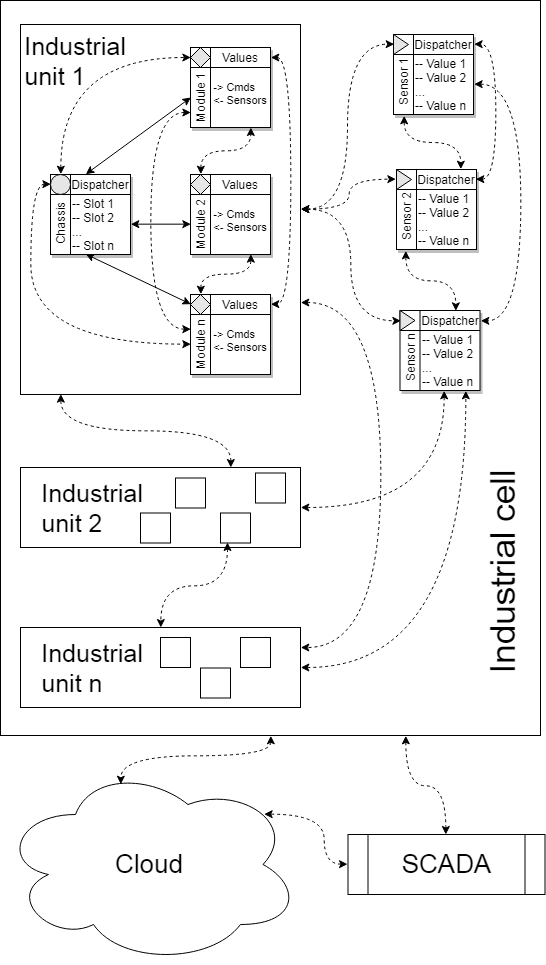
\includegraphics[width=0.5\textwidth]{ch-3/main-arch}
	}
	\caption*{Рисунок 1 "--- Слотовая модель модульного оборудования}\label{fig:main-arch}
\end{figure}

Предлагается следующая процедура инициализации модулей при их подключении к диспетчеру. Физическое подключение каждого модуля реализуется по трехпроводному интерфейсу, где по двум проводникам передается питающее напряжении, а третий используется в качестве линии безопасности (safety line). Линия безопасности объединяет все модули одной единицы оборудования по схеме монтажное И. В данной схеме линия безопасности подтянута резистором к плюсу питания. Так как сопротивление между линией и землей бесконечность, а между питанием и линией равно номиналу резистора, то напряжение на линии равно напряжению питания. То есть высокий уровень или логическая единица. Как уже было сказано выше, все модули подключены к линии и могут замыкать её на землю. Соответственно, на линии будет высокий уровень тогда и только тогда, когда все модули выставят высокий уровень на своих выходах. Как только любой из модулей соединит линию с землей, на ней установится низкий логический уровень и не один модуль не сможет на это повлиять.

Вновь подключенный модуль вначале осуществляет подключение к сети OpenThread, затем переводит линию безопасности на низкий логический уровень. Диспетчер детектирует это, после чего получает список всех ближайших к нему узлов (neighbors в терминологии OpenThread), выбирает среди них те, которые имеют статус не подключен, после чего просит первого из них перевести линию обратно на высокий логический уровень. Если уровень изменился, значит диспетчер и модуль подключены к одной линии, следовательно, модуль может быть зарегистрирован в реестре. В противном случае, диспетчер переходит к следующему модулю в списке.

Так как основной структурой хранения и передачи данных в системе является JSON, далее рассматривается методика определения максимальной пропускной способности канала передачи данных при передаче данных в данном в формате через очереди сообщений. Рассматриваются следующие сетевые сценарии:

\begin{enumerate}
	\item Взаимодействие процессов операционной системы
	\item Взаимодействие аппаратных и программных модулей в неоднородной компьютерной сети
	\item Взаимодействие с пользователем (оператором)	
\end{enumerate}

Далее описываются проведенные эксперименты. В качестве тестового оборудования выступили: персональный компьютер общего назначения (General PC), портативный компьютер (Laptop), высокопроизводительный сервер (сервер), облачный виртуальный сервер (Virtual server) и встраиваемая система (Microcomputer). Отмечается, что в экспериментах осуществлялась передача сообщений JSON в бинарном формате. В эксперименте участвовали следующие программные библиотеки бинаризации JSON: MessagePack, BSON, UBJSON, CBOR. В качестве очереди сообщений использовалась программная библиотека nanomsg.

Вначале было проведено сравнение пропускной способности сокетов TCP и UNIX. Отмечено, что по результатам измерений лучший способ межпроцессного взаимодействия в POSIX-совместимых операционных системах "--- сокеты TCP. Далее были проведены измерения средней пропускной способности сетевых подключений. Данная часть эксперимента показала, что использование протокола HTTP приводит к появлению дополнительных накладных расходов, поэтому этот метод исключается из расчета средней пропускной способности. Затем была проведена оценка производительности бинарных упаковщиков JSON. Отмечается, что для всех библиотек практически не наблюдается зависимости степени сжатия от размера файла JSON. Затем была получена зависимость скорости упаковки/распаковки от размера файла JSON. Для всех рассмотренных библиотек эта зависимость линейная. Библиотека CBOR показала лучшее время как для упаковки, так и для распаковки.
Следующим шагом было тестирование производительности библиотек CBOR, написанных на разных языках программирования. Произошло 1000 циклов упаковки/распаковки; размер исходного файла JSON был 15\,МБ. Далее были произведены замеры пропускной способности протокола nanomsg. 

На основе полученных данных была проведена общую оценка производительности протокола очереди сообщений. Для этого предложена следующая формула (1): 

\begin{equation}
\begin{split}
\label{eq:example}
\mathcal{B}_a = \frac{\mathcal{M}}{t}
= \frac{\mathcal{M}}{t_p + t_t + t_u}
= \frac{\mathcal{M}}
{\mathcal{M} / \mathcal{S}_p + 
	\gamma\mathcal{M} / \mathcal{B}_t + 
	\mathcal{M} / \mathcal{S}_u} = \\
= \frac{\mathcal{M}}
{\frac{\mathcal{M}_(\mathcal{B}_t\mathcal{S}_u) +
		\gamma
		\mathcal{M}(\mathcal{S}_p\mathcal{S}_u) +
		\mathcal{M}(\mathcal{S}_p\mathcal{B}_t)} 
	{\mathcal{S}_p\mathcal{B}_t\mathcal{S}_u}
}
=\frac{\mathcal{S}_p\mathcal{B}_t\mathcal{S}_u}
{\mathcal{B}_t\mathcal{S}_u + \gamma\mathcal{S}_p\mathcal{S}_u + \mathcal{S}_p\mathcal{B}_t}\,,
\end{split}
\end{equation}

\noindent где ${\mathcal{M}}$ "--- размер сообщения, $t$ "--- общее время между двумя точками, $t_p$ "--- время упаковки, $t_t$ "--- время передачи, $t_u$ "--- время распаковки, $\mathcal{S}_p$ "--- скорость упаковки данных JSON, $\mathcal{S}_u$ "--- скорость распаковки данных JSON, $\mathcal{B}_t$ "--- пропускная способность очереди сообщений, $\gamma$ "--- степень сжатия JSON.

Часто библиотеки Python демонстрируют производительность, примерно равную производительности библиотек C. Это связано с тем, что эти библиотеки являются просто оболочками библиотек C. В этом случае использование библиотек Python предпочтительнее из-за более простого синтаксиса языка программирования Python. Однако рассматриваемые библиотеки Python не показали достаточной производительности, поэтому очевидно, что для реализации серверной части была выбрана библиотека C. При реализации клиентской части использовалась библиотека JS, так как это единственный вариант реализации программ в браузере.

В таблице~1 показаны результаты расчетов. Расчеты показывают, что средняя полоса пропускания описанного канала связи находится в диапазоне от \SI{6}{\percent} (наихудший случай, упаковка/распаковка требуется на обеих конечных точках) до \SI{145}{\percent} (лучший случай, упаковка/распаковка вообще не требуется, обе конечные точки используют двоичные данные JSON, что подразумевает возможность сжатия сообщений из-за того, что двоичный формат JSON занимает меньше места по сравнению с текстовым JSON).

\begin{table}[!htb]
	\centering
	\caption*{Таблица 1 "--- Пропускная способность, кабельное соединение, $\gamma=0,65$}
	\label{tab:res}
	\begin{IEEEeqnarraybox} [\IEEEeqnarraystrutmode \IEEEeqnarraystrutsizeadd{2pt}{0pt}]{x/u/Vx/r/v/r/v/r/x/}
	\IEEEeqnarraydblrulerowcut \\
	
	& \hfill %\raisebox{0pt}[0pt][0pt]{Отношение $\mathcal{S}_u / \mathcal{S}$}
	\hfill && \IEEEeqnarraymulticol{0}{h}{}%
	\IEEEeqnarraystrutsize{0pt}{0pt} \\
	
	&&&& \hfill \raisebox{0pt}[0pt][0pt]{Библиотека JS} \hfill &&
	\hfill \raisebox{0pt}[0pt][0pt]{Библиотека C} \hfill &&
	\hfill \raisebox{0pt}[0pt][0pt]{Без распаковки} \hfill &
	\IEEEeqnarraystrutsizeadd{0pt}{2pt} \\
	%
	\IEEEeqnarraydblrulerowcut \\
	
	& Библиотека JS &&& n/a \rlap{\textsuperscript{1}} && {57.06} && 70.94 & \\
	& &&& &&{(6.22\,\%)} && (7.60\,\%) & \\
	
	& Библиотека  C &&& 67.50 && 117.70 && 203.18 & \\
	& &&& (7.24\,\%) && (12.62 \,\%) && (21.78 \, \%) & \\
	
	& Без упаковки &&& 93.31 && 227.27 && {1354.98} & \\
	& &&& (10.00\,\%) && (24.37\,\%) && {(145.28\,\%)} & \\
	%
	\IEEEeqnarraydblrulerowcut \\
	& \IEEEeqnarraymulticol{9}{s}{\scriptsize\textsuperscript{1} Cвязь между клиентами не реализована в рассматриваемом сценарии.}%
	\end{IEEEeqnarraybox}
\end{table}

Далее в главе отмечается, что наиболее узким местом в рассматриваемой информационной модели является передача данных по беспроводному каналу в условиях промышленного производства. Поэтому рассматривается методика оценки качество соединения при использовании модулей беспроводной связи, в частности оценено влияние факторов производственной среды, которые могут привести к ухудшению связи. Отмечается, что тестирование будет проводиться в частотном диапазоне \SI{2,4}{\giga\hertz}, так как этот диапазон является наиболее распространённым в потребительских сетях передачи данных: Wi-fi, Bluetooth и т.\,д. 

Отмечается, что за метрику качестве передаваемого сигнала принимается параметр RSSI, так как получение данного параметра не требует применения специальной измерительной техники (анализаторов спектра). Более того, в подавляющем большинстве потребительских радиомодулей, рассчитанных на частоту \SI{2,4}{\giga\hertz}, этот параметр рассчитывается автоматически. Также предложено использовать дополнительную метрику $RSSI_T$, основанную на характеристиках антенн, учитывающего свойства антенн и затухание сигнала~\cref{eq-1, eq-2, eq-3}:

\begin{equation}
RSSI_T = A-10 \mu\log (d),
\label{eq-1}
\end{equation}

\noindent где $d$ "--- расстояние от источника, м; $\mu$ "--- показатель ослабления, $\mu = 2$;

\begin{equation}
A = P_{out} + G_{tx} + G_{rx} -FSPL,
\label{eq-2}
\end{equation}

\noindent где $P_{out}$ "--- выходная мощность передатчика, дБм; $G_{tx}$ "--- усиление исходной антенны, дБи; $G_{rx}$ "--- усиление антенны приемника, дБи; $FSPL$ "--- потери на трассе в свободном пространстве, дБ;

\begin{equation}
FSPL = 10 \log (d) +20 \log (f) +20 \log (4 \pi/c),
\label{eq-3}
\end{equation}

\noindent где $f$ "--- частота, Гц; $c = 299792458$ м/с.

Поэтому в предлагаемом методе используется отклонение $\Delta RSSI$, полученное как разница между измеренным значением $RSSI_P$ и теоретическим значением $RSSI_T$~ \cref{eq-4}.

\begin{equation}
\Delta RSSI = RSSI_T-RSSI_P
\label{eq-4}
\end{equation}

Далее выдвигается гипотеза о том, что, если при проектировании беспроводной сети вначале определяются местоположение узлов в помещении, то логично можно перейти от метрики $\Delta RSSI$ к максимальному расстоянию между узлами~$D_{max}$~\cref{eq-5}, более удобному параметру для рассматриваемой задачи. Сигнал со значением RSSI менее~-80\,дБм считается слабым. На основе этой гипотезы и~\cref{eq-4} можно рассчитать метрику $RSSI_T$~\cref{eq-6} на определенном расстоянии от передатчика с учетом среднего отклонения $\Delta RSSI$, на которую влияют факторы конкретной производственной среды~\cref{eq-7}.

\begin{equation}
D_{max} = 10^\frac{A-RSSI_T}{10 \mu}
\label{eq-5}
\end{equation}

\begin{equation}
RSSI_T = -80-\overline{{\mathit \Delta} RSSI}
\label{eq-6}
\end{equation}

\begin{equation}
\overline{{\mathit \Delta} RSSI} = \frac1n \sum_{\substack{0 < i < n}}{\mathit\Delta} RSSI_i,
\label{eq-7}
\end{equation}

\noindent где $n$ "--- количество измерений. В этом случае $n = 25$.  

Далее описывается ряд экспериментов, проводимых в реальных производственных условиях.д о том, что многие производственные факторы оказывают существенное влияние на качество сигнала в беспроводной сети. Однако воздействие недостаточно  В качестве радиомодуля был использован чип nRF52840, были проведены измерения для различных факторов, влияющих на сигнал. По результатам экспериментов сделан вывовелико, чтобы отказываться от применения этой технологии. Более того, влияние многих факторов может быть сокращено за счет использования топологии ячеистой сети и плотного расположения приемников и передатчиков. Особо отмечается важность проведения соответствующих измерений для каждого конкретного производства, поскольку это обеспечивает эффективное размещение приемников и передатчиков в производственных помещениях. Также указывается, что полученные результаты особенно интересны в контексте оцифровки производства, где беспроводной метод передачи данных от датчиков становится предпочтительнее проводного из-за требований гибкости и мобильности производственного процесса. 


\textbf{В четвёртой главе} приведено описание процесса реализация модульной платформы технологического оборудования. Постулировано, что модульная технологическая платформа (сокр.~\textit{МТП}) является экспериментальным комплексом, построенным на основании подходов и методик, описанных в предыдущих главах. Описаны области применения подобного модульного оборудования, в частности, рассмотрены сценарии применения в мелкосерийном и единичном производстве. Далее рассмотрены конструктивные особенности МТП. Показано, что конструктивно состоит из универсального шасси~(сокр. ~\textit{УШ}), которое снабжено координатным столов с кареткой, на подвесе которой размещаются сменные модули. 

Рассматриваются различные конструкции, которые могут быть применены для создания УШ. На основании сравнительного анализа в качестве базовой конструкции шасси предлагается использование декартовой платформы с подвижным порталом, реализующим перемещение в плоскости XY. При этом отмечается, что для многих видов оборудования, которое может быть реализовано на базе МТП, не требуется дополнительная Z координата, поэтому эта координата в МТП является опциональной и может устанавливаться при необходимости.

Далее проводится анализ существующих приводов, которые могут быть использованы при создании УШ. Рассматриваются такие виды линейных приводов, как линейный шаговый двигатель, цепная передача, передачи на основе зубчатых ремней, а также шарико-винтовые  и ролико-винтовые передачи. Также рассматриваются различные виды направляющих, по которым будет осуществляться линейное перемещение, в частности, рассматриваются варианты с рельсовыми направляющими различных типов и направляющие на основе гладких цилиндрических валов. На основе сравнительного анализа достоинств и недостатков всех рассмотренных решений в качестве конструкции линейных приводов УШ предлагается использование шарико-винтовых передач с гладкими цилиндрическими направляющими.

После выбора конструкции линейных приводов приводится анализ существующих электродвигателей, рассматриваются два основных типа электродвигателей: редукторные серводвигатели и шаговые двигатели. Выделяется рад критериев для сравнения, по результатам которого предпочтение отдается шаговым двигателям. Следующим этапом описывается окончательная электрокинематическая схема координатного стола УШ~(рисунок~2).

\begin{figure}[ht]
	\centerfloat{
		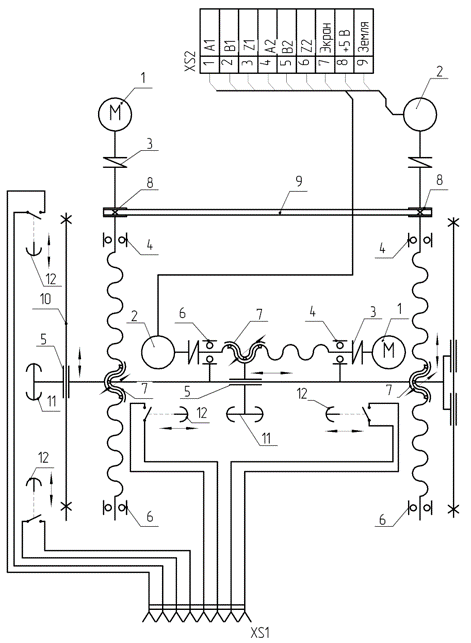
\includegraphics[width=0.7\textwidth]{ch-4/el-mech-sch}
	}
	\caption*{Рисунок 2 "--- Электрокинематическая схема координатного стола УШ: 1 "--- двигатель шаговый, 2 "--- датчик угла поворота, 3 "--- муфта кулачковая, 4 "--- Подшипник радиальный, 5 "--- подшипник линейный, 6 "--- Подшипник радиальный, 7 "--- ШВП, 8 "--- Шкив зубчатый, 9 "--- Ремень зубчатый, 10 "--- Направляющая, 11 "--- Щелевой оптический датчик, 12 "--- Выключатель концевой}\label{fig:scheme}
\end{figure}

Заключительный раздел главы посвящен описанию разработки универсального блока управления УШ. УШ является центральным компонентом МТП, так как позволяет связать аппаратную часть создаваемого на базе этой концепции оборудования (занимается получением данных от датчиков УШ и рабочих органов, генерирует управляющие сигналы приводов) и программную часть (связывает оборудование с ПК и позволяет осуществлять двухсторонний обмен данными с МТП). Универсальный блок управления состоит из следующих модулей:

\begin{itemize}
\item Модуль питания.
\item Процессорный модуль.
\item Модуль сопряжения с ПК.
\item Модуль сопряжения с датчиками.
\item Модули управления приводами.
\item Модуль индикации и взаимодействия с оператором.
\end{itemize}

Все модули будут снабжены собственным микроконтроллером, обеспечивающим их взаимодействие по протоколу SPI\footnote{сокр.~от~англ. англ. \textit{Serial Peripheral Interface, SPI bus.} "--- последовательный периферийный интерфейс, шина SPI.} Данный протокол позволит всем модулям соединяться между собой и обмениваться необходимой информацией в синхронном последовательном режиме. То есть универсальный блок управления представляет собой сеть микроконтроллеров, обеспечивающих различные функции. 

\FloatBarrier                      
\textbf{Заключение}.
%% Согласно ГОСТ Р 7.0.11-2011:
%% 5.3.3 В заключении диссертации излагают итоги выполненного исследования, рекомендации, перспективы дальнейшей разработки темы.
%% 9.2.3 В заключении автореферата диссертации излагают итоги данного исследования, рекомендации и перспективы дальнейшей разработки темы.

Значимость полученных в диссертационной работе результатов подчеркивается возможностью интеграции разработанных методик, подходов и алгоритмов в систему автоматизированного проектирования модульного технологического оборудования. Предложенные рекомендации по созданию узлов и агрегатов, а также блоков управления модульным технологическим оборудованием упростят его разработку и применение в условиях единичного и мелкосерийного производства.  В ходе исследования получены следующие основные теоретические и практические результаты:

\begin{enumerate}
  \item Предложена универсальная конструкция переналаживаемого модульного оборудования, состоящая из универсального координатного шасси с подвижной кареткой; модулей, определяющих основную операцию выполняемую оборудованием и устанавливаемых на подвесе каретки шасси посредством электромагнитного крепления; и модульного блока управления, реализующего алгоритм числового программного управления. 
  \item Разработано алгоритмическое и программно-техническое обеспечение модульного блока управления, включающее в себя набор программно-аппаратных средств для реализации децентрализованного сетевого взаимодействия модулей в проводной и беспроводной среде передачи данных и программное обеспечение для автоматической реконфигурации единицы модульного оборудования, позволяющее снизить трудоёмкость переналадки.  
  \item Разработана методика унификации модулей с электромагнитным креплением, включающая в себя способ определения параметров унификации и их ограничений и способ формирования параметрического ряда на основании сформулированных ограничений.
  \item Предложен критерий целесообразности применения модульного оборудования, основанный на анализе групповых технологических процессов, позволяющий оценить  перспективы использования модульного оборудования для типовых технологических процессов, используемых на предприятии.
  \item Разработана методика оптимизации комплекта модульного оборудования, включающая в себя способ расчёта весовых коэффициентов целевой функции оптимизации и алгоритм двухкритериальной оптимизации, основанный на теории нормирования и дискретно-событийном методе.
  \item На основании методики оптимизации комплекта модульного оборудования разработано программное обеспечение и проведен численный эксперимент, показавший повышение производительности производства группы изделий на~\SI{18}{\percent}.
  \item Для тестирования предложенной конструкции модульного оборудования, а также методик и алгоритмов работы с ним создан прототип модульной технологической платформы.
\end{enumerate}

Таким образом, на основании полученных результатов, цель данного диссертационного исследования по разработке модульного технологического оборудования для условий единичного и мелкосерийного производства можно считать достигнутой.

Полученные результаты соответствуют пункту 6 <<Разработка, исследование и внедрение новых видов технологического оборудования для изготовления деталей, сборки, регулировки, контроля и испытаний приборов>> и пункту 7 <<Разработка и внедрение новых методов и средств механизации, автоматизации, роботизации приборостроительного производства, обеспечивающих повышение производительности, снижение трудоемкости и повышение экономичности производства>> паспорта специальности 05.11.14 "--- <<Технология приборостроения>>.


\ifdefmacro{\microtypesetup}{\microtypesetup{protrusion=false}}{} % не рекомендуется применять пакет микротипографики к автоматически генерируемому списку литературы
\urlstyle{rm}                     % ссылки URL обычным шрифтом
\ifnumequal{\value{bibliosel}}{0}{% Встроенная реализация с загрузкой файла через движок bibtex8
  \renewcommand{\bibname}{\large \bibtitleauthor}
  \nocite{*}
  \insertbiblioauthor           % Подключаем Bib-базы
  %\insertbiblioexternal   % !!! bibtex не умеет работать с несколькими библиографиями !!!
}{% Реализация пакетом biblatex через движок biber
  % Цитирования.
  %  * Порядок перечисления определяет порядок в библиографии (только внутри подраздела, если `\insertbiblioauthorgrouped`).
  %  * Если не соблюдать порядок "как для \printbibliography", нумерация в `\insertbiblioauthor` будет кривой.
  %  * Если цитировать каждый источник отдельной командой --- найти некоторые ошибки будет проще.
  %
  %% authorconf
  \nocite{confbib-2017-trajectory-problems}%
  \nocite{confbib-2017-json}%
  \nocite{confbib-2017-modular-integration}%
  \nocite{confbib-2017-machine-vision}%
  \nocite{confbib-2017-microservices}%
  \nocite{confbib-2018-motion-profile}%
  \nocite{confbib-2018-etherium}%
  \nocite{confbib-2018-mesh}%
  \nocite{confbib-2018-blockchain}%
  \nocite{confbib-2019-interpolation}%
  \nocite{confbib-2019-voice-assistant}%
  \nocite{vakbib-wpan-2020}%
  \nocite{confbib-2020-smart-controller}%
  \nocite{confbib-2020-auto-positioning}%
  \nocite{confbib-2020-RSSI}
  %
  %% authorvak
  \nocite{vakbib-microservice-2018}%
  \nocite{vakbib-blockchain-2019}%
  \nocite{vakbib-machine-vision-2020}%
  %
  %% authorwos
  %\nocite{wosbib1}%
  %
  %% authorscopus
  %\nocite{scbib1}%
  %
  %% authorpathent
  %\nocite{patbib1}%
  %
  %% authorprogram
  %\nocite{progbib1}%
  %
  %% authorother
  %\nocite{bib1}%
  %\nocite{bib2}%

  \ifnumgreater{\value{usefootcite}}{0}{
    \begin{refcontext}[labelprefix={}]
      \ifnum \value{bibgrouped}>0
        \insertbiblioauthorgrouped    % Вывод всех работ автора, сгруппированных по источникам
      \else
        \insertbiblioauthor      % Вывод всех работ автора
      \fi
    \end{refcontext}
  }{
  \ifnum \totvalue{citeexternal}>0
    \begin{refcontext}[labelprefix=A]
      \ifnum \value{bibgrouped}>0
        \insertbiblioauthorgrouped    % Вывод всех работ автора, сгруппированных по источникам
      \else
        \insertbiblioauthor      % Вывод всех работ автора
      \fi
    \end{refcontext}
  \else
    \ifnum \value{bibgrouped}>0
      \insertbiblioauthorgrouped    % Вывод всех работ автора, сгруппированных по источникам
    \else
      \insertbiblioauthor      % Вывод всех работ автора
    \fi
  \fi
  %  \insertbiblioauthorimportant  % Вывод наиболее значимых работ автора (определяется в файле characteristic во второй section)
  \begin{refcontext}[labelprefix={}]
      \insertbiblioexternal            % Вывод списка литературы, на которую ссылались в тексте автореферата
  \end{refcontext}
  % Невидимый библиографический список для подсчёта количества внешних публикаций
  % Используется, чтобы убрать приставку "А" у работ автора, если в автореферате нет
  % цитирований внешних источников.
  \printbibliography[heading=nobibheading, section=0, env=countexternal, keyword=biblioexternal, resetnumbers=true]%
  }
}
\ifdefmacro{\microtypesetup}{\microtypesetup{protrusion=true}}{}
\urlstyle{tt}                               % возвращаем установки шрифта ссылок URL
